\chapter{Evaluation}

Dieses Kapitel beschreibt die finale Evaluation der HoloLens Planner App mit Handwerkern. Zu erst wird die Durchführung erklärt und anschließend die gewonnenen Erkenntnisse aus Fragebogen und den nachfolgenden Gesprächen. Dabei wird genauer darauf eingegangen, wie gebrauchstauglich die Applikation den Handwerkern erscheint, wie sie die Belastung bei ihrer Benutzung einschätzen, ob sie die Technologie Augmented Reality zur Unterstützung ihrer Arbeit in Zukunft akzeptieren würden, wie sie die Erfahrung mit der Applikation fanden und wie man diese noch entwickeln könnte. Es wurden sieben verwertbare Fragebögen und zehn Interviews erzeugt.

\section{Durchführung der Evaluation}

Die Tests wurden bei zehn Handwerkern einzeln, an unterschiedlichen Tagen, zu Hause mit der Microsoft HoloLens und der HoloLens Planner Applikation durchgeführt. Zur Ausführung der Tests wurde den Handwerkern anfangs grob der Umfang dieser Masterarbeit erklärt und was damit bezweckt wird. Anfangs wurde durch Literaturrecherche der aktuelle Stand der Digitalisierung in Handwerksbetrieben und KMUs festgestellt. Um die Materie der Arbeit auf dem Bau kennenzulernen und im Beruf eines Handwerkers Erfahrungen zu machen, die vorher nicht bestanden, wurde eine Ethnographie zum Handwerk des Fliesenlegers durchgeführt. Dadurch wurden Ansatzpunkte für die Unterstützung durch Technologie, genauer durch die Nutzung von Augmented Reality, für Fliesenleger gefunden. Aus diesen Funden wurde eine AR Applikation für die Microsoft HoloLens entwickelt, welche Handwerker beim Kundengespräch, durch virtuelles Fliesenverlegen, sowie beim Fliesen verlegen, durch einblenden eines blauen Rasters helfen soll. Diese Applikation gilt es nun mit Handwerkern zu testen und ihre Meinung darüber zu erheben. 

Die Daten wurden in 3 Phasen erhoben. 

\begin{itemize}
	\item Testen der Applikation in einem vordefinierten Szenario
	\item Ausfüllen des Fragebogens
	\item Unstrukturiertes Gespräch
\end{itemize}

Zum Testen wurde jeweils eine große, freie Fläche benötigt. Den Probanden wurde das Szenario erst erklärt und anschließend wurden sie durch die Applikation geleitet. Es ging darum einen viereckigen Boden im Raum zu markieren und Fliesen darauf zu verlegen, den Verlegeassistenten zu aktivieren und Daten über die Fläche auszulesen. Erst platzierte jeder Proband vier Eckpunkte im Raum. Diese mussten nicht zwingend in tatsächlichen Ecken platziert werden, da das teilweise aus Platzgründen auch nicht möglich war. Nachdem die Fläche so markiert wurde, wählte sie eine Fliese aus, die sie verlegen wollten. Breite und Länge dieser konnten sie beliebig modifizieren. Anschließend legten sie sie auf dem abgesteckten Boden aus. Es wurde ihnen Zeit gegeben sich im Raum zu bewegen und das Bild aufzunehmen. Anschließend aktivierten sie den Verlegeassistenten, welcher nur die Fugen in blau auf dem Boden anzeigt. Wieder hatten sie Zeit, um sich mit dem Feature auseinander zu setzen. Zuletzt öffneten sie erneut das Bodenmenü und bekamen die Daten Fläche, Umfang und Anzahl der Fliesen angezeigt. Damit war der Test beendet.

Von da ging es direkt, ohne viel Kommunikation zum Fragebogen über, den sie freiwillig ausfüllen sollten. Dabei wurde ihnen nur kurz erklärt, wie dieser auszufüllen war. Unterstützt wurden sie dabei nur, wenn ihnen ein Wort undeutlich war. Ansonsten wurde dabei nicht geredet und sie füllten den Fragebogen selbstständig aus.

Zum Abschluss wurde ein unstrukturiertes Gespräch mit jedem Probanden geführt. Dabei sollten diese einfach über ihre Gedanken zu dem Experiment sprechen. Falls das Gespräch stagnierte wurde es mit Fragen, wie zum Beispiel \enquote{Was fanden Sie gut an der Applikation}, \enquote{Welche Funktionalitäten würden Sie sich noch wünschen} oder \enquote{Was hat Ihnen an der Applikation nicht gefallen} wieder angekurbelt. Generell waren die Handwerker jedoch gut im Redefluss und brachten viele eigene Ideen ein und dachten die bisherige Idee weiter. Diese Gespräche wurden, nach Absprache mit den Probanden, teilweise aufgezeichnet. Während jeder Unterhaltung wurden Notizen angefertigt, welche die Aussagen der Handwerker indirekt festhielten.

\section{Diskussion der Ergebnisse}

Diese Sektion zeigt die Ergebnisse der, durch die Handwerker, ausgefüllten Fragebögen. Alle Daten die hier aufgezeigt werden beziehen sich auf die sieben verwertbaren Fragebögen, die korrekt ausgefüllt wurden. 

\begin{figure}[h]
	\begin{center}
		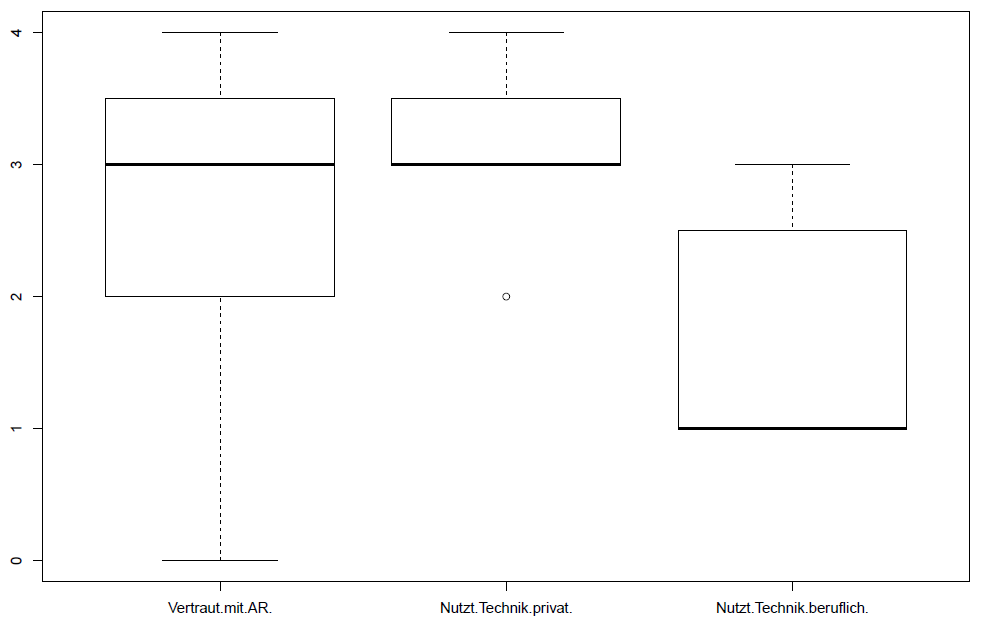
\includegraphics[scale=0.5]{Resources/Evaluation/allgemein.png}
		\label{allgemein}
		\caption{Erhobene allgemeine Daten}	
	\end{center}
\end{figure}

\begin{figure}[h]
	\begin{center}
		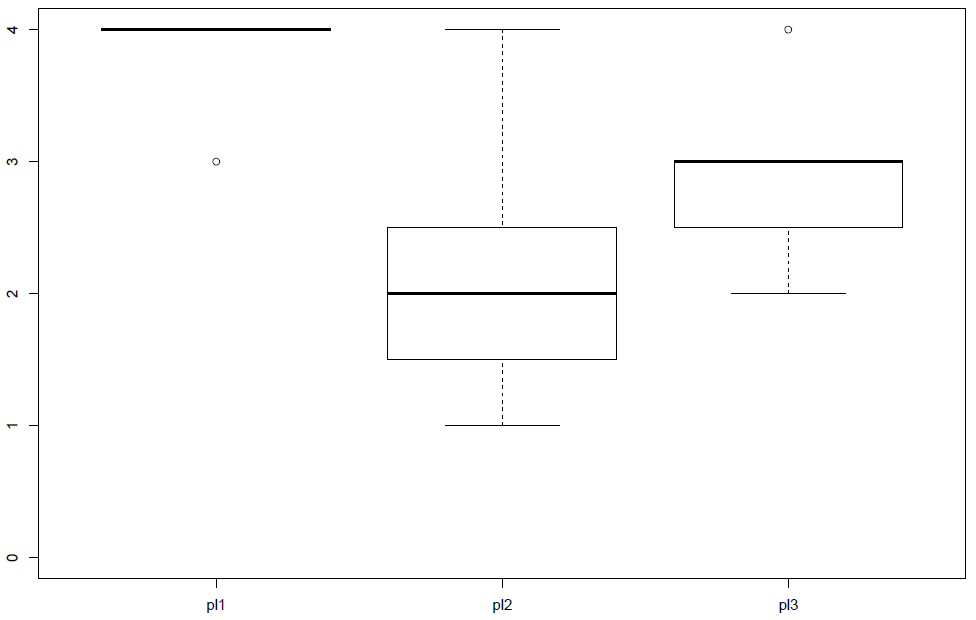
\includegraphics[scale=0.5]{Resources/Evaluation/playful.png}
		\label{playful}
		\caption{Erhobene Daten zur Playfulness}	
	\end{center}
\end{figure}

Alle Probanden waren männlich und zwischen 21 - 54 Jahre, fünf davon unter 40 Jahre und zwei über 40 Jahre, alt. Durchschnittlich gaben sie an mit der Technologie Augmented Reality gut vertraut zu sein. Das könnte auf die weite Verbreitung von VR in den letzten Jahren zurückzuführen sein und darauf, dass man diese Technologien häufig auf Messen oder sogar in Museen ausprobieren kann. Allerdings reichen die Angaben von nicht bis sehr vertraut. Im privaten Umfeld nutzen die Handwerker häufig technologische Hilfsmittel, im beruflichen hingegen eher weniger häufig (siehe Abbildung \ref{allgemein}). Das könnte ein weiteres Indiz sein, dass die Digitalisierung im Handwerk noch nicht weit fortgeschritten ist.

pl1 gibt an, dass die Nutzung von HoloLens Planner die Neugier aller Probanden stark anregt (siehe Abbildung \ref{playful}). Dieser Wert kann jedoch auf die Applikation selbst, als auch auf die Nutzung von AR generell bezogen sein. Augmented Reality stellt für die Handwerker zwar eine bekannte Technologie dar (siehe Abbildung \ref{allgemein}), jedoch wurde nicht erfragt, wie viele von ihnen schon eine VR oder AR Brille ausprobiert hatten. Die Probanden gaben an, dass sie nur mäßig die Zeit vergessen, während sie mit der Applikation arbeiteten. Nur ein Proband gab den höchsten Wert an, was sich mit seiner Aussage, er tauche komplett in die Erfahrung mit der Datenbrille ein abgleicht. Die teilweise Zustimmung, dass sie Freude am Arbeiten mit dem HoloLens Planner haben, lässt auf einen hohen Akzeptanzwert schließen.

Privat nutzt jeder Handwerker mindestens Computer und Smartphone. Über die Hälfte der Probanden gaben an auch von Tablets und teilweise Smartwatches Gebrauch zu machen. Das kann darauf hindeuten, dass sie technisch versiert sind und erklärt auch, warum sie die Nutzung der Microsoft HoloLens schnell, nach einmaligem Erklären, verstanden und umsetzen konnten. \\
Beruflich nutzen über die Hälfte der Handwerker Computer und Smartphone. Einzelne Probanden gaben an nur den Computer oder nur eine Smartphone zu nutzen. Knapp die Hälfte der Probanden setzen auch Tablets in ihrem Beruf ein und einer davon auch eine Smartwatch. Interessant ist, dass zwei der Handwerker Laser zum vermessen nutzen. Laut ihren Aussagen ermöglichen diese ihnen die Messungen noch genauer vorzunehmen, Messfehlern vorzubeugen und so auch besonders kleine Fugen von unter 3mm präzise und konsistent legen zu können. Das nur zwei der sieben Handwerker Laser verwenden kann darauf hindeuten, dass noch kein Großteil der Handwerker alle Möglichkeiten an technischen Hilfsmitteln, welche momentan verfügbar sind, zu ihrem Vorteil nutzen.

Die nächsten Abschnitte zeigen die Auswertung der psychologisch getesteten Fragen aus \ref{fragebogen}. Aussagen der Handwerker aus den Interviews fließen dabei mit ein und helfen die Ergebnisse zu interpretieren.

\subsection{Gebrauchstauglichkeit}

Mit Hilfe der SUS wird bestimmt, wie Gebrauchstauglich und Benutzerfreundlich die Handwerker den HoloLens Planner fanden. \\
Der Durchschnittswert aller SUS Wertungen beträgt 85\% (siehe Abbildung \ref{sus_allBox}). Laut \cite{rauer_quantitative_2011} bedeutet das für die Applikation eine gute bis exzellente Usability. Insgesamt konnten die Handwerker die Applikation also gut bedienen und empfanden diese als nicht zu kompliziert, was dafür sprechen kann, sie auch in ihren Arbeitsalltag zu integrieren. Wie Krcmar \cite{hateful_six_krcmar} schon feststellte, ist eine einfache Bedienung und Gebrauchstauglichkeit ein entscheidender Faktor, ob eine neue Technologie akzeptiert wird oder nicht. Dieses Ergebnis deutet positiv in diese Richtung. \\
Alle Probanden bis auf zwei werteten die Usability des HoloLens Planners vergleichsweise hoch, das heißt mit einem Wert von 80 oder mehr (siehe Abbildung \ref{sus_all}). Dabei handelt es sich um die Probanden unter 30 Jahren. Diese sind mit mehr technischen Medien aufgewachsen und könnten daher einen besseren Zugang zu neuen Technologien, wie Augmented Reality haben. Die beiden Ausreißer, SUS-Wert 72,5 und 65, stammen von den Probanden über 40. Es wurde bereits erwartet, dass für diese die Bedienung der Microsoft HoloLens und der Applikation schwerer ist. Die Daten deuten darauf hin, dass diese Vermutung stimmt. Allerdings kann man bei einer kleinen Versuchsmenge von sieben Personen nicht genau sagen, ob das der Fall ist. 

\begin{figure}[h]
	\begin{center}
		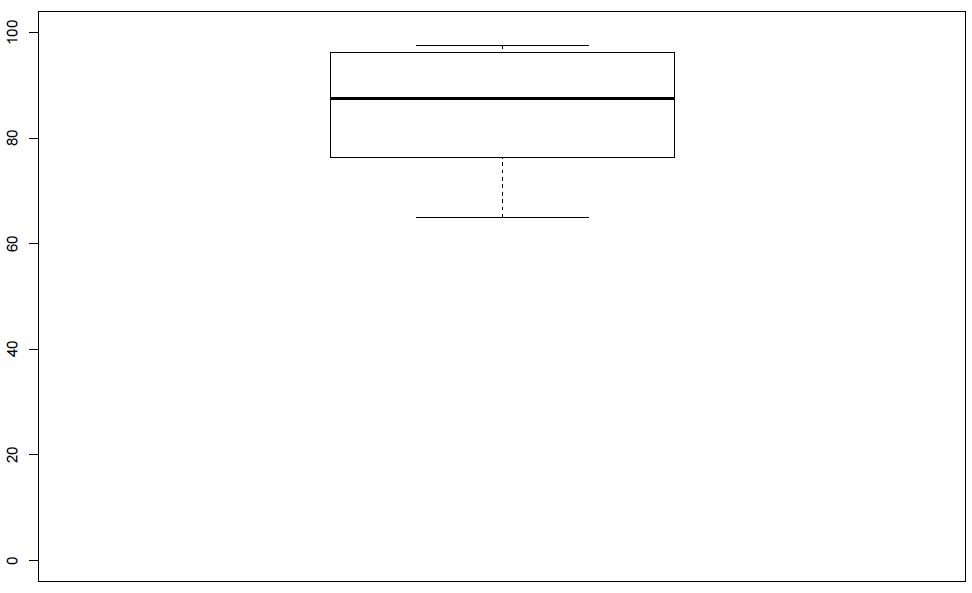
\includegraphics[scale=0.5]{Resources/Evaluation/sus_totalBox.png}
		\label{sus_allBox}
		\caption{Verteilung der SUS-Werte}	
	\end{center}
\end{figure}

\begin{figure}[h]
	\begin{center}
		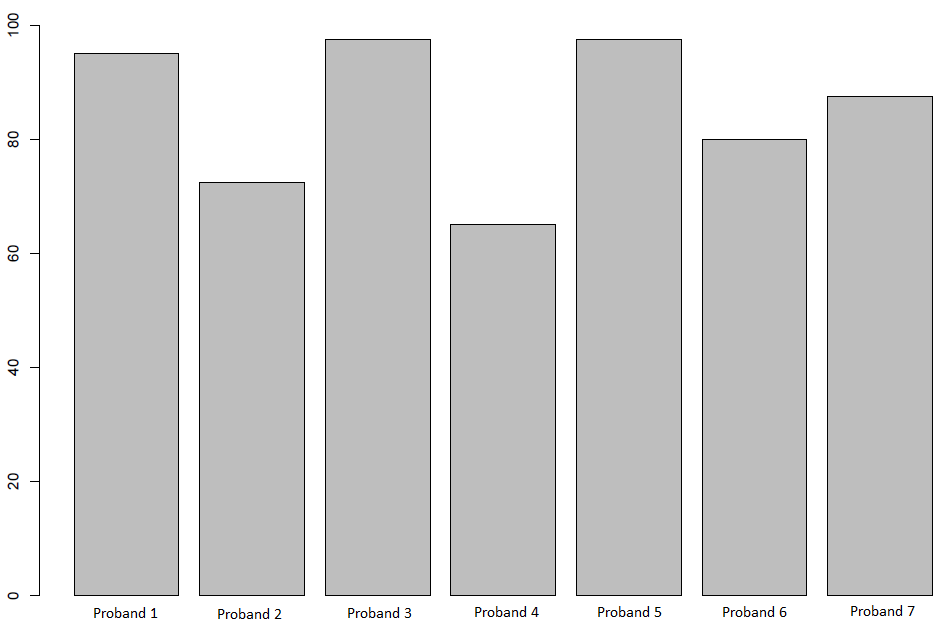
\includegraphics[scale=0.5]{Resources/Evaluation/sus_allTotals.png}
		\label{sus_all}
		\caption{SUS der einzelnen Probanden}	
	\end{center}
\end{figure}

\begin{figure}[H]
	\begin{center}
		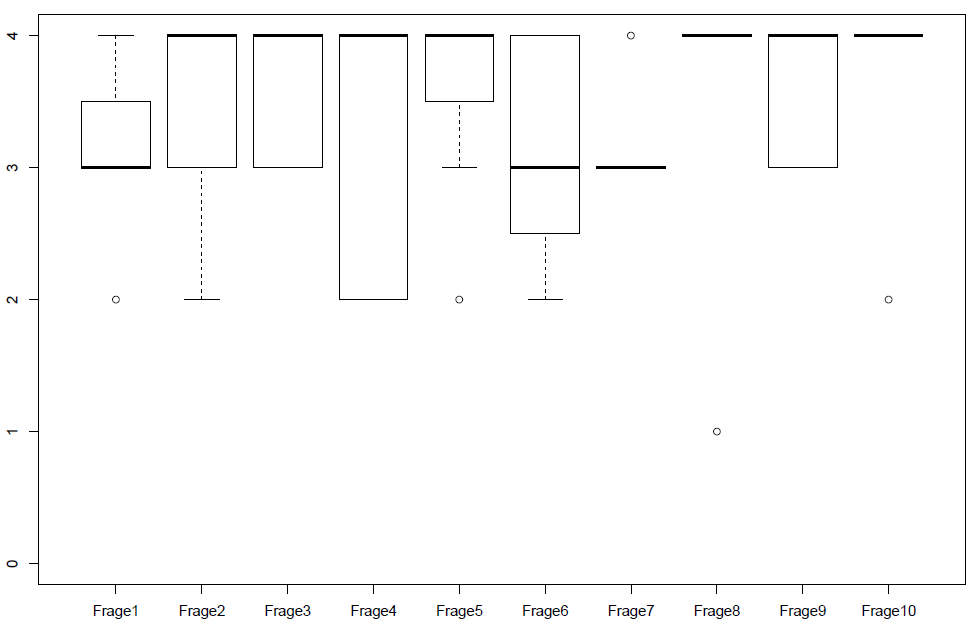
\includegraphics[scale=0.5]{Resources/Evaluation/sus_allQuestionsBox.png}
		\label{sus_questionsBox}
		\caption{Verteilungen der Antworten auf die einzelnen Fragen der SUS}	
	\end{center}
\end{figure}

In Abbildung \ref{sus_questionsBox} fallen Besonderheiten bei den Fragen 5, 8 und 10 auf. \\
Bei Frage 5 gaben alle Probanden bis auf zwei volle Punktzahl. Beide sind über 40 Jahre alt und dadurch wahrscheinlich technisch weniger versiert und äußern ihre Meinung kritischer. Die Angabe des Probanden, welcher die Frage mit 2 Punkten bewertete, passt zu seinen Aussagen im Interview, wo er angibt, dass das blaue Raster zu ungenau sei und dass es definitiv ein Problem sei, dass es nicht mehr eingeblendet wird, wenn er zu nahe ran gehe. Der andere Proband ist, laut Interview, sehr mit der Applikation zufrieden. Eine Abweichung von einem Punkt hat auch keine große Aussagekraft. \\
Das alle Probanden voll Punktzahl gaben, bis auf Proband 4, der nur einen Punkt gab bei Frage 8, fällt deutlich auf. Dabei ist Interessant, dass der Handwerker im Interview angab, dass er sich mit der App sehr vertraut fühle, die Bedienung jedoch als umständlich empfand. Das könnte allerdings nur auf die Funktionalitäten und Möglichkeiten bezogen sein, nicht auf die Bedienung selbst. Diese könnte ihm schwer fallen, da er zu den älteren Probanden zählt. Der andere Handwerker über 40 wiederum gab volle Punktzahl. Er verwendet jedoch bei der Arbeit auch Laser und könnte daher mit technischen Neuerungen besser zurecht kommen. \\
Bei Frage 10 gaben auch alle Probanden bis auf Nummer 4 volle Punktzahl. Hier ist die Vermutung, dass er sich damit auf die Erklärung der Funktionalitäten vor dem Test bezog und auf die Eingewöhnungsphase. Proband 2, welcher auch über 40 Jahre alt ist und angab nicht mit AR vertraut zu sein gab hier wiederum volle Punktzahl. Daraus lässt sich also leider kein guter Schluss ableiten.

\subsection{Arbeitsbelastung}

Mithilfe des NASA-TLX wurde die empfundene Arbeitsbelastung der Handwerker beim Nutzen der HoloLens Planner Applikation gemessen. Mit einem Durchschnittswert von ca. 25 von 100 ist die Belastung eher gering einzuschätzen (siehe Abbildung \ref{nasa_all}). Da AR eine relativ neue und unbekannte Technologie ist, wurde erwartet, dass dieser Wert durchaus höher ist. Interessant ist dabei, dass die Probanden 2 und 4, die über 40 Jährigen, Belastungswerte über 30 angaben. Damit lässt sich aber keine auf das Alter bezogene Aussage machen, da Probanden 1, 5 und 6 auch höhere Werte über 25 aufweisen (siehe Abbildung \ref{nasa_allWorkloads}). Proband 7, einer der jüngsten der relativ wenig Technologie in der Arbeit nutzt, kam auf einen Wert unter 10 und damit auf den niedrigsten. Insgesamt lässt sich damit jedoch sagen, dass die Nutzung der Applikation und AR für die Handwerker wenig anstrengend seien könnte, was positiv für den weiteren Einsatz von AR ist. Da hier mit dem ungewichteten NASA-TLX gearbeitet wurde, muss mehr ins Detail gegangen werden, um bessere Aussagen treffen zu können.

\begin{figure}[h]
	\begin{center}
		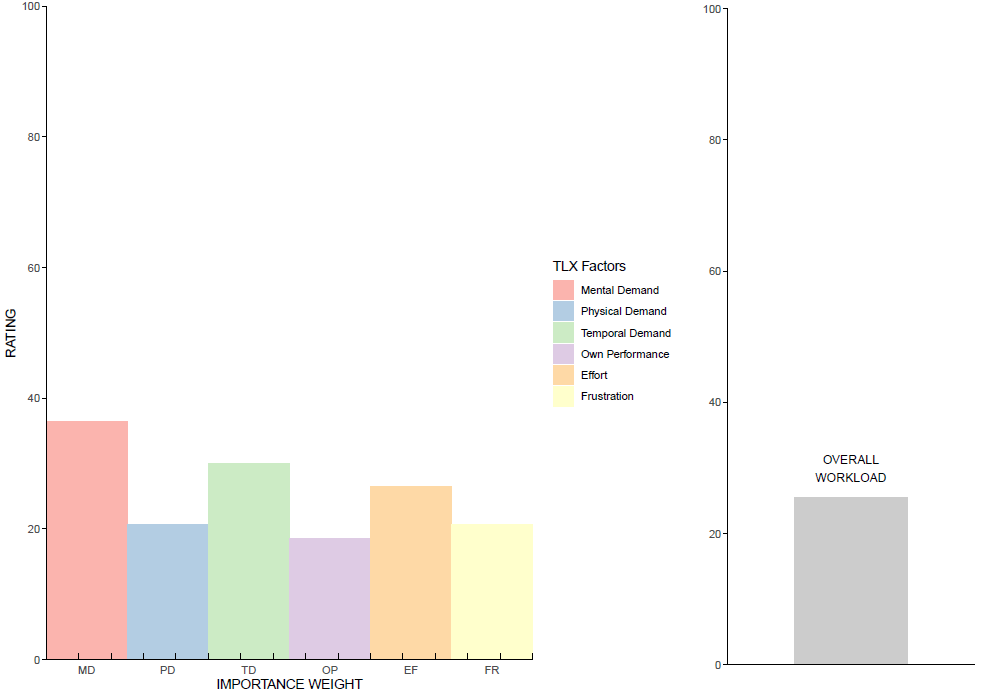
\includegraphics[scale=0.5]{Resources/Evaluation/nasa_all.png}
		\label{nasa_all}
		\caption{Mittelwerte aller Antworten und der Arbeitsbelastung}	
	\end{center}
\end{figure}

\begin{figure}[h]
	\begin{center}
		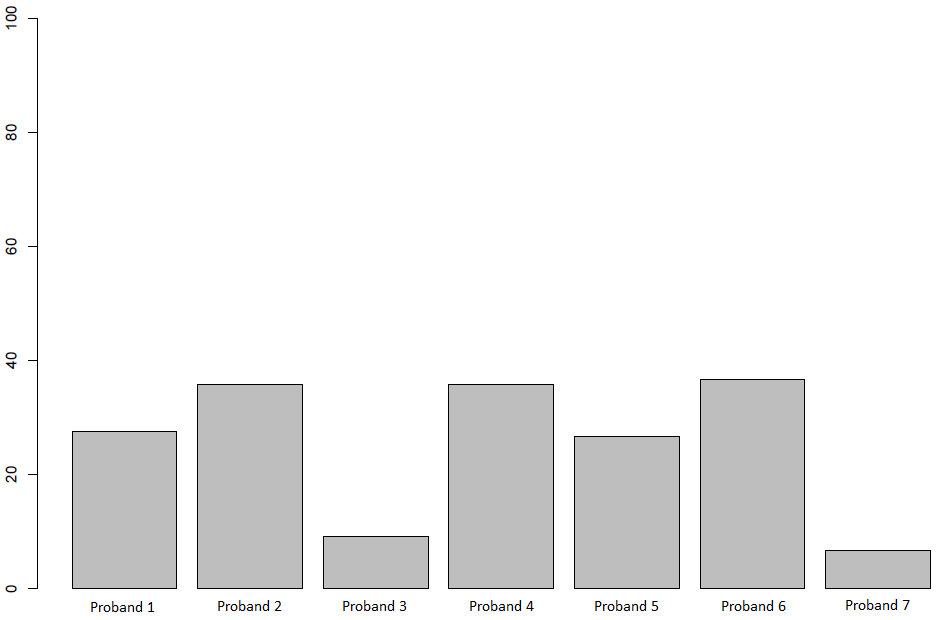
\includegraphics[scale=0.5]{Resources/Evaluation/nasa_allWorkloads.png}
		\label{nasa_allWorkloads}
		\caption{Verteilung aller Ergebnisse für Arbeitsbelastung}	
	\end{center}
\end{figure}

Die Geistige Anforderung fiel mit einem Durchschnittswert von 36 am höchsten aus (siehe Abbildung \ref{nasa_questions}). AR könnte also mental fordernd seien und den Arbeitern bei der Nutzung auf dem Bau so viel Aufmerksamkeit abverlangen, welche sie dann nicht mehr auf ihre Umgebung richten können. Proband 1 gab dazu an, dass man stark in die Erfahrung mit der Datenbrille eintaucht und so nicht mehr genau wahrnimmt, was um einen herum passiert. Die HoloLens blendet das Umfeld jedoch nicht aus, wie eine VR Brille, weshalb man dieses Phänomen weiter untersuchen sollte. Proband 5 gab an, dass die Applikation das Ausmessen vereinfachen würde, jedoch stimme die Perspektive nicht immer ganz, wodurch man Umdenken muss. Das könnte seine hoch empfundene mentale Belastung erklären. Die Brille sei noch zu unpraktisch und lenke dadurch von der Tätigkeit ab, war die Aussage von Proband 6.

Die Werte für körperliche Anforderung bleiben unter 50 (siehe Abbildung \ref{nasa_questions}), sind gut verteilt und weisen einen Mittelwert von 20 auf. Dadurch lässt sich schließen, dass das Nutzen von AR mental deutlich anspruchsvoller sein könnte als physikalisch. Dies war jedoch anzunehmen. Proband 4 ist hier der einzige Ausreißer mit einem Wert von 45. Dies könnte jedoch auf sein Alter zurückzuführen sein, da er angab, die Verwendung der Applikation fühle sich vertraut an.

Es wurde angenommen, dass die Applikation den Zeitaufwand deutlich verringert. Jedoch empfanden die Handwerker die aufgebrachte Zeit für das Testszenario als nicht gering mit den meisten Werten im Bereich zwischen 30 und 50 (siehe Abbildung \ref{nasa_questions}). Insgesamt stellt diese Dimension mit einem Durchschnittswert von 30 die zweitgrößte Belastung dar. Dies ist eventuell auf das Erstmalige verwenden einer neuen Technologie zurückzuführen. Die Probanden 3 und 7 empfanden den Zeitaufwand jedoch als sehr gering und bestätigten im Interview auch, dass sich mit der Applikation Zeit sparen ließe. Dies müsste in wiederholten Tests geprüft werden.

Mit der Erbrachten Leistung waren alle Handwerker zufrieden, was der Durchschnittswert von 19 bestätigt (siehe Abbildung \ref{nasa_questions}). Das gleicht sich mit den Aussagen, dass alle sich vorstellen könnten, dass die Technologie Vorteile bringt, ab. Es lässt sich also vermuten, dass die Arbeitsleistung damit verbessert oder zumindest unterstützt werden könnte. Alle Werte sind gut verteilt zwischen 0 und 35. Proband 2, welcher die Wertung 35 abgab, war von dem blauen Raster zur Verlegeunterstützung nicht überzeugt, wodurch sich dieser Wert erklären ließe.

Die Probanden empfanden die Erfahrung mit der Applikation und der Datenbrille als mäßig anstrengend, was der Mittelwert von 26 zeigt (siehe Abbildung \ref{nasa_questions}). Die Probanden 2 und 4 bewerteten es als anstrengend mit einem Wert über 40. Für sie schien die Nutzung aber generell anstrengender zu sein als für andere Probanden. Handwerker 1 empfand es auch als anstrengend, was sich mit seiner Aussage, dass er sich stark auf die Brille und die Arbeit damit konzentrieren müsse, abgleicht. Interessant sind die Aussagen von Proband 3 und 6, welche sehr gering ausfielen. Sie gaben auch an, das die Applikation leicht zu bedienen sei und ihre Arbeit erleichtern würde.

Die Frustration mit der Applikation hielt sich in Grenzen bei einem Durchschnittswert von 20. Nur Proband 6, mit einem ungewöhnlich hohen Wert von 80 stach hervor (siehe Abbildung \ref{nasa_questions}). Die Angabe scheint hoch, dafür dass er die Bedienung relativ einfach fand und sich vorstellen konnte, dass die App seine Arbeit erleichtert. Er hält die Technologie jedoch noch für unpraktisch und nicht alltagstauglich, was den hohen Wert erklären könnte. 

\begin{figure}[h]
	\begin{center}
		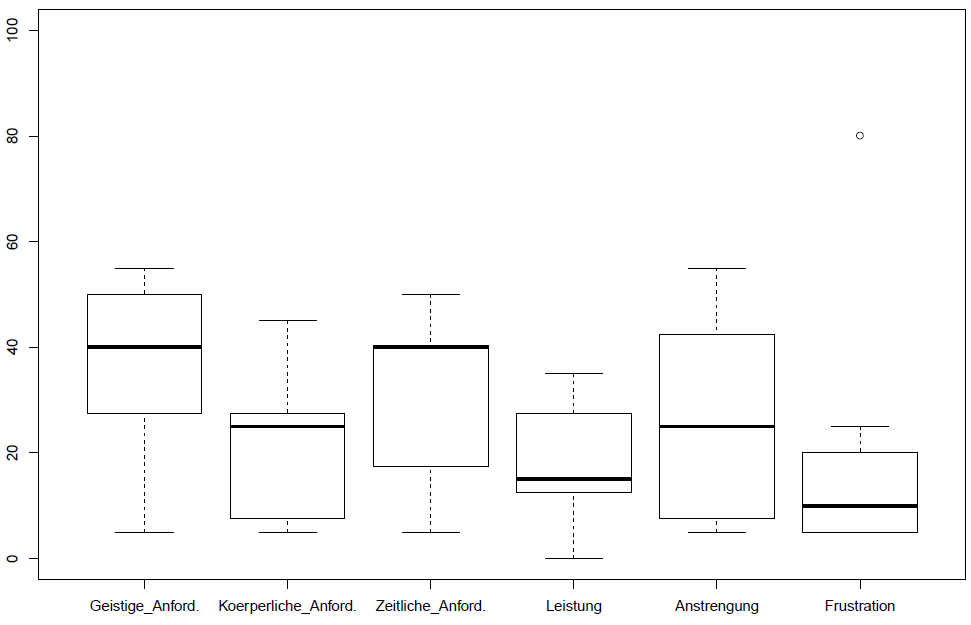
\includegraphics[scale=0.5]{Resources/Evaluation/nasa_questions.png}
		\label{nasa_questions}
		\caption{Verteilung der Antwortwerte der einzelnen Fragen}	
	\end{center}
\end{figure}

\subsection{Akzeptanz der neuen Technologie}

Dieser Abschnitt wertet die Angaben der Handwerker zu den Fragen des TAM Models aus. Dabei wird zwischen den beiden Features zur Unterstützung beim Kundegespräch und dem Verlegeassistenten unterschieden. Items, welche ein \enquote{x} im Namen tragen zählen zu Ersterem, Items mit einem \enquote{y} im Namen zu Zweiterem. Die Wahrgenommene Einfachheit wurde auf die gesamte Applikation gemessen, da sich diese auf die Bedienung, welche durch die Gestensteuerung der Microsoft HoloLens begrenzt ist, und nicht die Güte der einzelnen Features bezieht. Insgesamt bewerteten die Probanden die Applikation als sehr einfach zu nutzen.

\subsubsection{Unterstützung beim Kundengespräch}
\label{kunde_show}

\begin{figure}[h]
	\begin{center}
		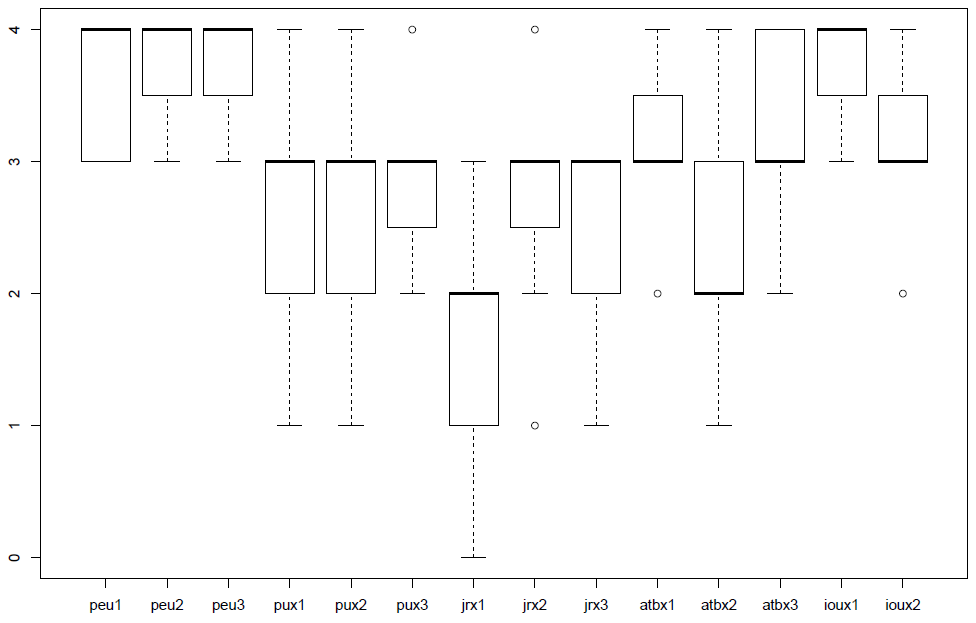
\includegraphics[scale=0.5]{Resources/Evaluation/tam_show.png}
		\label{tam_show}
		\caption{Kundengespräch: Verteilung der Antworten der einzelnen Items}	
	\end{center}
\end{figure}

\begin{figure}[H]
	\begin{center}
		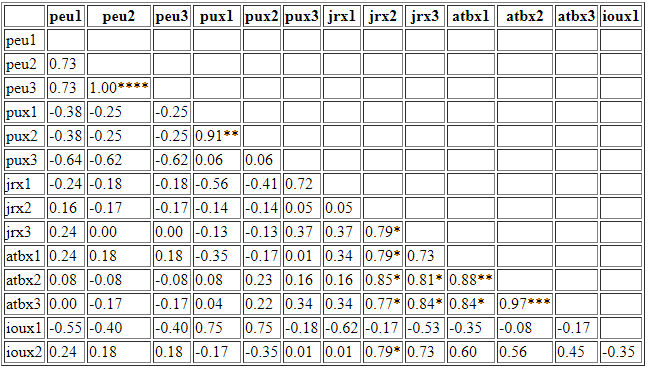
\includegraphics[scale=0.7]{Resources/Evaluation/cor_show.png}
		\label{tam_showCor}
		\caption{Kundengespräch: Korrelation der Items}	
	\end{center}
\end{figure}

Die Handwerker stufen das Feature als nützlich führ ihre Arbeit ein. Da aus der Fokusgruppe und der Ethnographie hervorging, dass das Kundengespräch eines der größten Probleme im Handwerk darstellt und ein Visualisierungswerkzeug Abhilfe schaffen könnte, war das anzunehmen. Die kleine Datenmenge ließ es jedoch nicht zu einen Bezug zwischen der gut empfundenen Relevanz für den Beruf und der wahrgenommenen Nützlichkeit einen aussagekräftigen Zusammenhang zu finden. Diese Relevanz wirkt sich positiv auf die Einstellung der Handwerker zu dem Feature aus. In Abblidung \ref{tam_showCor} zeigt sich eine signifikante Korrelation zwischen der Relevanz für den Beruf und der Einstellung der Handwerker zur Unterstützung beim Kundengespräch. Zusätzlich zeigt die Korrelation zwischen \enquote{jrx2} und \enquote{ioux2}, dass Handwerker die Unterstützung wahrscheinlicher nutzen würden, wenn sie sie als relevant für ihren Beruf sehen. Die Einstellung der Handwerker zur Visualisierungsfunktion ist gut mit Tendenz zu sehr gut. Sehr wahrscheinlich würden die Probanden das Werkzeug nutzen, wenn sie die Möglichkeit dazu hätten. Aus den Korrelationen ergibt sich, dass dieser Effekt verstärkt wird, wenn sie das Tool für Relevant für ihre Arbeit halten. Insgesamt zeigen die Ergebnisse, dass das Visualisierungswerkzeug für das Kundengespräch für gut empfunden wird und das Potential besitzt tatsächlich genutzt zu werden (siehe Abbildung \ref{tam_show}).

\subsubsection{Unterstützung beim Fliesenlegen}
\label{kunde_assist}

\begin{figure}[h]
	\begin{center}
		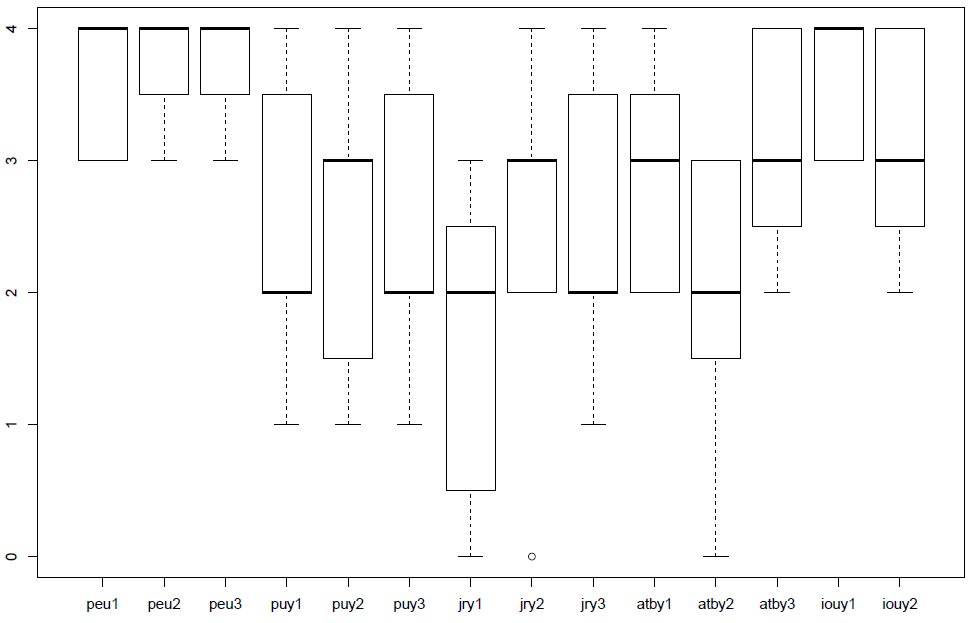
\includegraphics[scale=0.5]{Resources/Evaluation/tam_assist.png}
		\label{tam_assist}
		\caption{Verlegeassistent: Verteilung der Antworten der einzelnen Items}	
	\end{center}
\end{figure}

Laut Abbildung \ref{tam_assist} sehen die Handwerker dieses Feature als mäßig bis gut nützlich an. Im Vergleich zu dem Visualisierungswerkzeug ist das etwas geringer, was zu Beginn der Tests auch so angenommen wurde. Handwerker vertrauen eher auf ihr handwerkliches Können, als auf Assistenzsysteme. Dies zeigt sich auch in den Daten zur Job Relevanz. Diese wird von den Probanden als mäßig angegeben, was darauf schließen ließe, dass sie nicht viel Potential zur Zeitersparnis beim Fliesenverlegen sehen. Die Job Relevanz hat einen signifikanten Einfluss auf die wahrgenommene Nützlichkeit (siehe Abbildung \ref{tam_assistCor}). Die Einstellung der Handwerker gegenüber der Nutzung ist gut und höher als die beiden vorherigen Variablen (siehe Abblidung \ref{tam_assist}). Die wahrgenommene Nützlichkeit scheint dabei eine große Rolle zu spielen, was man aus den Korrelationen ableiten kann. Die Relevanz für die Arbeit hat einen deutlich signifikanten Einfluss - bis zu 0,001 - auf die Einstellung der Probanden zur Applikation. Um so wichtiger sie es also für ihre Arbeit halten, desto eher würden sie die Applikation nutzen. Trotz geringerer wahrgenommener Nützlichkeit sind die Handwerker dem Feature gegenüber gut eingestellt und würden es mit hoher Wahrscheinlichkeit nutzen, wenn sie Zugang dazu hätten (siehe Abbildung \ref{tam_assist}). Die wahrgenommene Nützlichkeit scheint darauf einen signifikanten Einfluss zu haben. Insgesamt scheint es, dass die Unterstützung beim Fliesenlegen gut bei den Handwerkern ankam und sie darin Potential für die Zukunft sehen.

\begin{figure}[h]
	\begin{center}
		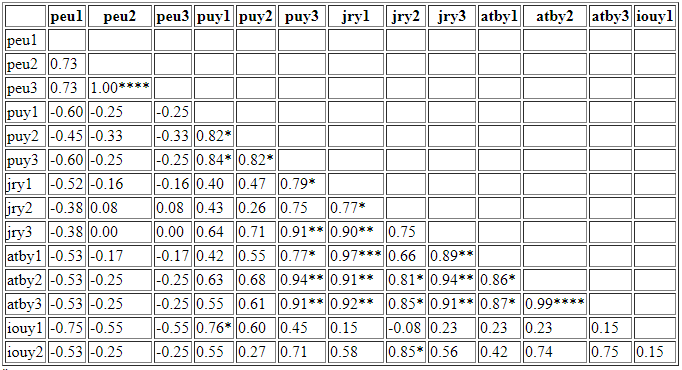
\includegraphics[scale=0.7]{Resources/Evaluation/cor_assist.png}
		\label{tam_assistCor}
		\caption{Verlegeassistent: Korrelation der Items}	
	\end{center}
\end{figure}

\section{Auswertung der Interviews}

Die Interviews geben Aufschluss über die Gedanken der Handwerker zu der Verwendung des HoloLens Planners und zu Augmented Reality. Sie beschreiben dabei, wie sie sich vorstellen könnten die Applikation in ihrem momentanen Zustand zu verwenden, aber auch ihre Visionen für AR für die Zukunft und was damit verbessert oder vereinfacht werden könnte. Im Folgenden sind ihre Aussagen zusammengefasst.

\subsection{Diskussion zur Intention die Applikation zu nutzen}

Die meisten Handwerker sind überzeugt davon, dass ihnen das virtuelle Fliesenverlegen bei Kundengesprächen weiterhelfen kann. Damit ist es möglich den Kunden zu zeigen, wie das Endergebnis aussehen kann. Ein Handwerker merkte an, dass diese es mit der Brille auch anderen Familienmitgliedern zeigen können. Bis jetzt hat er das immer über Referenzen, wie beispielsweise Bilder von anderen Baustellen gemacht. Mit der Applikation sieht der Kunde es direkt vor sich. Er kann auch verschiedene Farbkombinationen an Fliesen ausprobieren und so sehen, wie sich der Raum anfühlt. Das vereinfache das Kundengespräch. \\
Ein Problem kann dabei darstellen, dass nur eine Person die Brille tragen kann. Dies könnte die Diskussion über Einzelheiten und Änderungen wieder erschweren. Insgesamt sind die Handwerker mit dem Werkzeug sehr zufrieden und würden es gerne direkt anwenden, was sich auch in den iou-Werten des TAM (siehe \ref{kunde_show}) zeigt.

Ein weiteres Anwendungsfeld, welches bei der Entwicklung der Applikation nicht primär bedacht wurde, für welches die Handwerker die Applikation geeignet sehen, ist als Planungswerkzeug. Bei Absprachen mit anderen Handwerkern treten oft Verständigungsprobleme auf. Durch die Applikation könnte jeder Handwerker das geplante im Raum sehen, wodurch Anweisung klarer wären. \\
Die Probanden lobten, dass die Applikation bereits die Fläche und den Umfang des Raumes, sowie die Anzahl der benötigten Fliesen anzeigt. Durch die Quadratmeter ließe sich direkt der benötigte Kleber und durch die Anzahl der Fliesen die Fliesenpakete berechnen. Man kann mit der Applikation auch verwinkelte Räume abstecken, was schneller ginge, als diesen per Hand zu vermessen. All das seien wichtige Informationen für einen Fliesenleger, die er mit der Applikation in kürzester Zeit sammeln könne. Schlechten Verschnitt, wie beispielsweise Fliesen unter 2cm Breite könne er damit auch schon im voraus erkennen und bei der Planung bedenken. Dieses zusätzliche Potential, welches die Handwerker in dem Visualisierungswerkzeug sehen, könnte die guten Werte zu wahrgenommener Nützlichkeit in \ref{kunde_show} erklären. \\
Die Mehrheit der Probanden äußerten jedoch auch Bedenken zur Genauigkeit der Technologie. Teilweise stimmt die Perspektive nicht. Bei einem Test setzte ein Handwerker einen Punkt an eine Ecke im Raum. Aus seiner Sicht sah es korrekt aus. Als er sich jedoch an einen anderen Punkt stellte, schwebte der Eckpunkt versetzt zur Ecke und der Boden steckte teilweise in der Wand. Auch meinte ein Handwerker, die App könnte mit einem Laser nicht mithalten, welcher für sehr genaue Messungen eingesetzt wird. \enquote{Es geht um Millimeter}, sagte er, vor allem bei kleinen Fugen. Für eine grobe Planung und einen Überblick sei die Applikation jedoch sehr gut geeignet.

Zu dem blauen Raster, welches beim Verlegen der Fliesen unterstützen soll, gaben die Handwerker weniger Feedback. Sie könnten sich vorstellen, dass dies den Messaufwand verringern würde. Vor allem wenn eine Wand nicht im 90 Grad Winkel zur anderen steht, könnten sie das erkennen, da die Fliesenbreiten an dieser Wand auseinandergehen würden. Das blaue Raster würde dann ganz deutlich zeigen, ob Fliesen mit weniger als 2cm Breite benötigt würden. Mit dieser Information kann der Handwerker umplanen und ein besser angepasstes Muster verlegen. \\
Ein paar Probanden fanden das Raster jedoch zu dominant und als Verlegehilfe zu ungenau. Es würde verwirren, wenn man damit direkt arbeiten würde. Außerdem könne ein Fliesenleger durch das Stauchen und Strecken von Fugen viel ausgleichen, was von dem Raster nicht beachtet wird. Dies könnte die Werte zur wahrgenommenen Nützlichkeit erklären, welche bei \ref{kunde_assist} niedriger liegen, als bei \ref{kunde_show}. Insgesamt wären sie wahrscheinlich nicht abgeneigt es zu nutzen, wenn man die iou-Werte in \ref{kunde_assist} betrachtet.

Teilweise äußerten die Probanden auch Bedenken zur Microsoft HoloLens, welche mit der Applikation nichts zu tun hatten. Dabei bemängelten sie die Größe der Brille und ihr zerbrechliches Aussehen. Eine Baustelle ist eine harte Umgebung voller Staub und Dreck, in welcher die Datenbrille wahrscheinlich nicht lange überleben würde, besonders wenn man sie zum Arbeiten verwenden würde. Außerdem sei das Sichtfeld zu klein und der Nutzer müsse seinen Kopf sehr ruhig halten, um damit präzise zu Arbeiten. Diese Zeit bleibt dem Handwerker oft nicht. 

\subsection{Ideen und Erweiterungen}

Mit den Funktionalitäten der Applikation waren die Probanden recht zufrieden. Interessant ist auch, wie sie diese weiterdenken. 

Bei der Planung würde unterstützen meinte ein Handwerker, wenn die Wandlängen direkt eingeblendet würden. Zusätzlich sollte die Applikation die Winkel der Ecken bestimmen können. Dadurch lässt sich früh feststellen, ob eine Wand z.B. ungerade oder schlecht verputzt ist, was dazu führen kann, dass später Fliesen mit kleiner Breite benötigt werden. Die Applikation könnte auch den Verschnitt optimieren in dem sie beispielsweise verschiedene Verlegemöglichkeiten automatisch berechnet und zur Auswahl bereit stellt. Außerdem wäre es interessant, wenn in der Planung mit einberechnet wird, falls zum Beispiel an einer Seite eine halbe Fliese benötigt wird und auf der anderen Seite eine gedrittelte. Beide Stücke könnten aus einer Fliese geschnitten werden. Ein Proband meinte, Händler würden gerne die Fliesen schon vorgeschnitten liefern, sodass der Fliesenleger sie dann nur noch an entsprechender Stelle einlegen muss. Das wäre durch ein gutes Planungswerkzeug eventuell auch möglich. Das Verlegen sollte auch von verschiedenen Punkten aus funktionieren, damit man mit Mustern experimentieren kann.

Verschiedengroße Fliesen in Mustern zu kombinieren wäre für die neumodischen Wünsche der Kunden auch ein gefragtes Feature. Dabei sollte die Applikation mindestens verschiedene Verbände, wie beispielsweise den römischen Verband oder Halbverband abdecken. Auch wäre es nützlich, wenn Fliesen in Mustern unterschiedliche Farben annehmen könnten. 

Zur Unterstützung bei der Arbeit merkte eine Handwerker an, dass eine Schablone für das Zuschneiden der Fliesen hilfreich wäre. Es solle möglich sein einzelne Fliesen aus dem Muster herauszugreifen, deren Umriss wie eine Schablone auf eine physikalische Fliese zu projizieren und diese dann zurechtzuschneiden.

Eine weitere interessante und große Idee wäre das Koppeln des HoloLens Planners mit anderen Systemen. Um die Fliesenauswahl zu erweitern könnte man sie mit Fliesenkatalogen der Händler verbinden. So erhält man immer die neuesten Fliesenmodelle. Oder man könne eine physikalische Fliese mit der HoloLens fotografieren und deren Farbe direkt auf virtuelle Fliesen übertragen. Dadurch könnte der Kunde mehr mit den Farben experimentieren. \\
Viele der Handwerker merkten das Potential an, die Applikation mit einem CAD Programm zu kombinieren. Dabei könnte man den Ansatz verwenden, den Raum mit der HoloLens zu scannen und dieses Raumbild an ein CAD System am Computer zu senden und es dort einrichten. Oder der Fliesenleger gibt die genau gemessenen Daten in sein CAD System ein, richtet den Raum so her, wie er oder Kunde es wünscht und lädt das Ergebnis auf die HoloLens. Bei Kunden zu Hause projiziert die Datenbrille das Ergebnis in den Rohbau. Dieser kann sich dann frei darin bewegen und so erfahren, wie sich beispielsweise sein neues Bad anfühlen würde.

Die Probanden können sich auch gut vorstellen die Applikation nicht nur für Fliesenleger zu verwenden. Auch für Blechdachleger, Dachdecker, Parkettleger, Fassadenbauer und Innenarchitekten könnten sie sich eine AR Applikation dieser Art als nützlich vorstellen.

\section{Fazit}

Alle Probanden hatten eine gute Erfahrung beim Testen des HoloLens Planners auf einer AR Brille. Diese weist eine beinahe exzellente Gebrauchstauglichkeit auf, wobei diese von den jüngeren Probanden höher gewertet wurde, als von den älteren. Das könnte auf das Alter zurückzuführen sein, da die Jüngeren mit mehr Technologie aufwuchsen. Andererseits gaben die Älteren öfter kritische Antworten. Hierzu hätten noch mehr Daten zur technischen Versiertheit erhoben werden können. Die Ausführungszeit jedes Probanden für das Szenario und das Wissen, ob er bereits eine VR und/oder AR Brille ausprobiert hatte, könnte die SUS Ergebnisse noch besser erklären.

Damit eine Applikation besser in den Arbeitsalltag integriert werden kann, sollte sie nicht anstrengend zu nutzen sein, was durch den NASA-TLX Wert von 25 durchaus gegeben sein kann. Auch hier gaben die älteren Probanden einen höheren Wert an. Hauptsächlich sei die Applikation mental fordernd. Das kann dazu führen, das sie in der rauen Umgebung einer Baustelle weniger geeignet ist, da sie zu sehr vom Umfeld ablenkt. Es wurde angenommen, dass die Applikation den Zeitaufwand der Handwerker verringern kann. Ihre Einschätzung beim testen spricht allerdings dagegen. Dies könnte jedoch auf die geringe Erfahrung der Teilnehmer mit AR zurückzuführen sein. Es müssten mehr Tests durchgeführt werden, um darüber eine genaue Aussage machen zu können.

Es wurde erwartet, dass eine Unterstützung beim Kundengespräch interessant sein kann, wie aus der Fokusgruppe und der Ethnographie hervorgeht. Die Handwerker bestätigten dies im Fragebogen. Sie sind dem Visualisierungswerkzeug gegenüber positiv eingestellt, sehen es als relevant für ihre Arbeit und würden die Applikation, so wie sie ist bereits gerne nutzen, wenn das möglich wäre. \\
Für den Verlegeassistenten wurde angenommen, dass Handwerker diesen schlecht einstufen würden, da sie ihre Arbeit mit Augenmaß besser erledigen könnten. Sie sehen ihn zwar als weniger relevant und nützlich für ihre Arbeit, würden ihn aber trotzdem gerne nutzen. Auch wenn sie dieses Feature etwas schlechter bewerteten, könnte das bedeuten, dass sie eine Unterstützung bei der Arbeit durchaus begrüßen würden. Da die Probanden von AR generell begeistert waren könnte dieser Wert auch daher rühren, dass sie generell gerne AR nutzen würden. \\
Um diese Antworten nochmal zu evaluieren hätte es hilfreich sein können, die Handwerker im Interview zu fragen, wie anstrengend sie die Erfahrung und wie gut sie die einzelnen Features fanden.

Die Handwerker würden gerne das Visualisierungstool nutzen, um Kunden ihre Pläne zu zeigen, damit Farbkombinationen zu testen und ein besseres Kundegespräch führen zu können. Auch für die Planung würden sie sie gerne nutzen, um die Räume schnell zu vermessen und den Verschnitt zu optimieren. Zu dem Raster äußerten sich die Handwerker im Interview wenig aber positiv, was die Zahlen auch unterstützen. Es könnte also ein gewünschtes Feature sein, welches bei der Arbeit hilft. \\
Einige Kritik erntete die HoloLens selbst. Sie sei zu unhandlich, zu instabil und das Sichtfeld wäre nicht groß genug. Das mache sie für den Einsatz auf der Baustelle ungeeignet. Dem könnte mit einer Datenbrille Abhilfe geschafft werden, welche speziell für solche Szenarien entwickelt wurde. Insgesamt würden sie die Applikation jedoch gerne nutzen.

Das zeigte sich auch darin, dass die Handwerker sich bereits beim Testen Gedanken über die Zukunft der Applikation machen. Sie würden Funktionalitäten zur Vermessung der Winkel begrüßen, sowie eine automatische Verschnittoptimierung, welche ihnen verschiedene Muster mit wenig Verschnitt zur Auswahl bereit stellt. Eine Schablone zum Zuschneiden der Fliesen wurde auch gewünscht. Die Kombination der AR Brille mit einer CAD Software beschrieben sie als bestes Feature, welches ihnen einige Vorteile bringen könnte. Diese Applikation könne dann auch für andere Handwerker genutzt werden und sei nicht nur auf Fliesenleger beschränkt.